\section{연구 과정}

\subsection{천체망원경 모터 초점 조절 장치 컨트롤러 제작}

\subsubsection{회로도 제작}

천체망원경 모터 초점 조절 장치 컨트롤러를 제작하기 위해서는 위에서 나열한 대로의 여러 가지 부품들이 필요할 것이다. 하지만 이러한 부품들의 개수가 많아질수록 회로도가 복잡한 정도는 기하급수적으로 늘어나기 때문에 여러 프로그램의 도움을 받아 회로도를 그리는 것이 일반적인 방법이다.
\begin{wrapfigure}{l}{0.5\textwidth}
	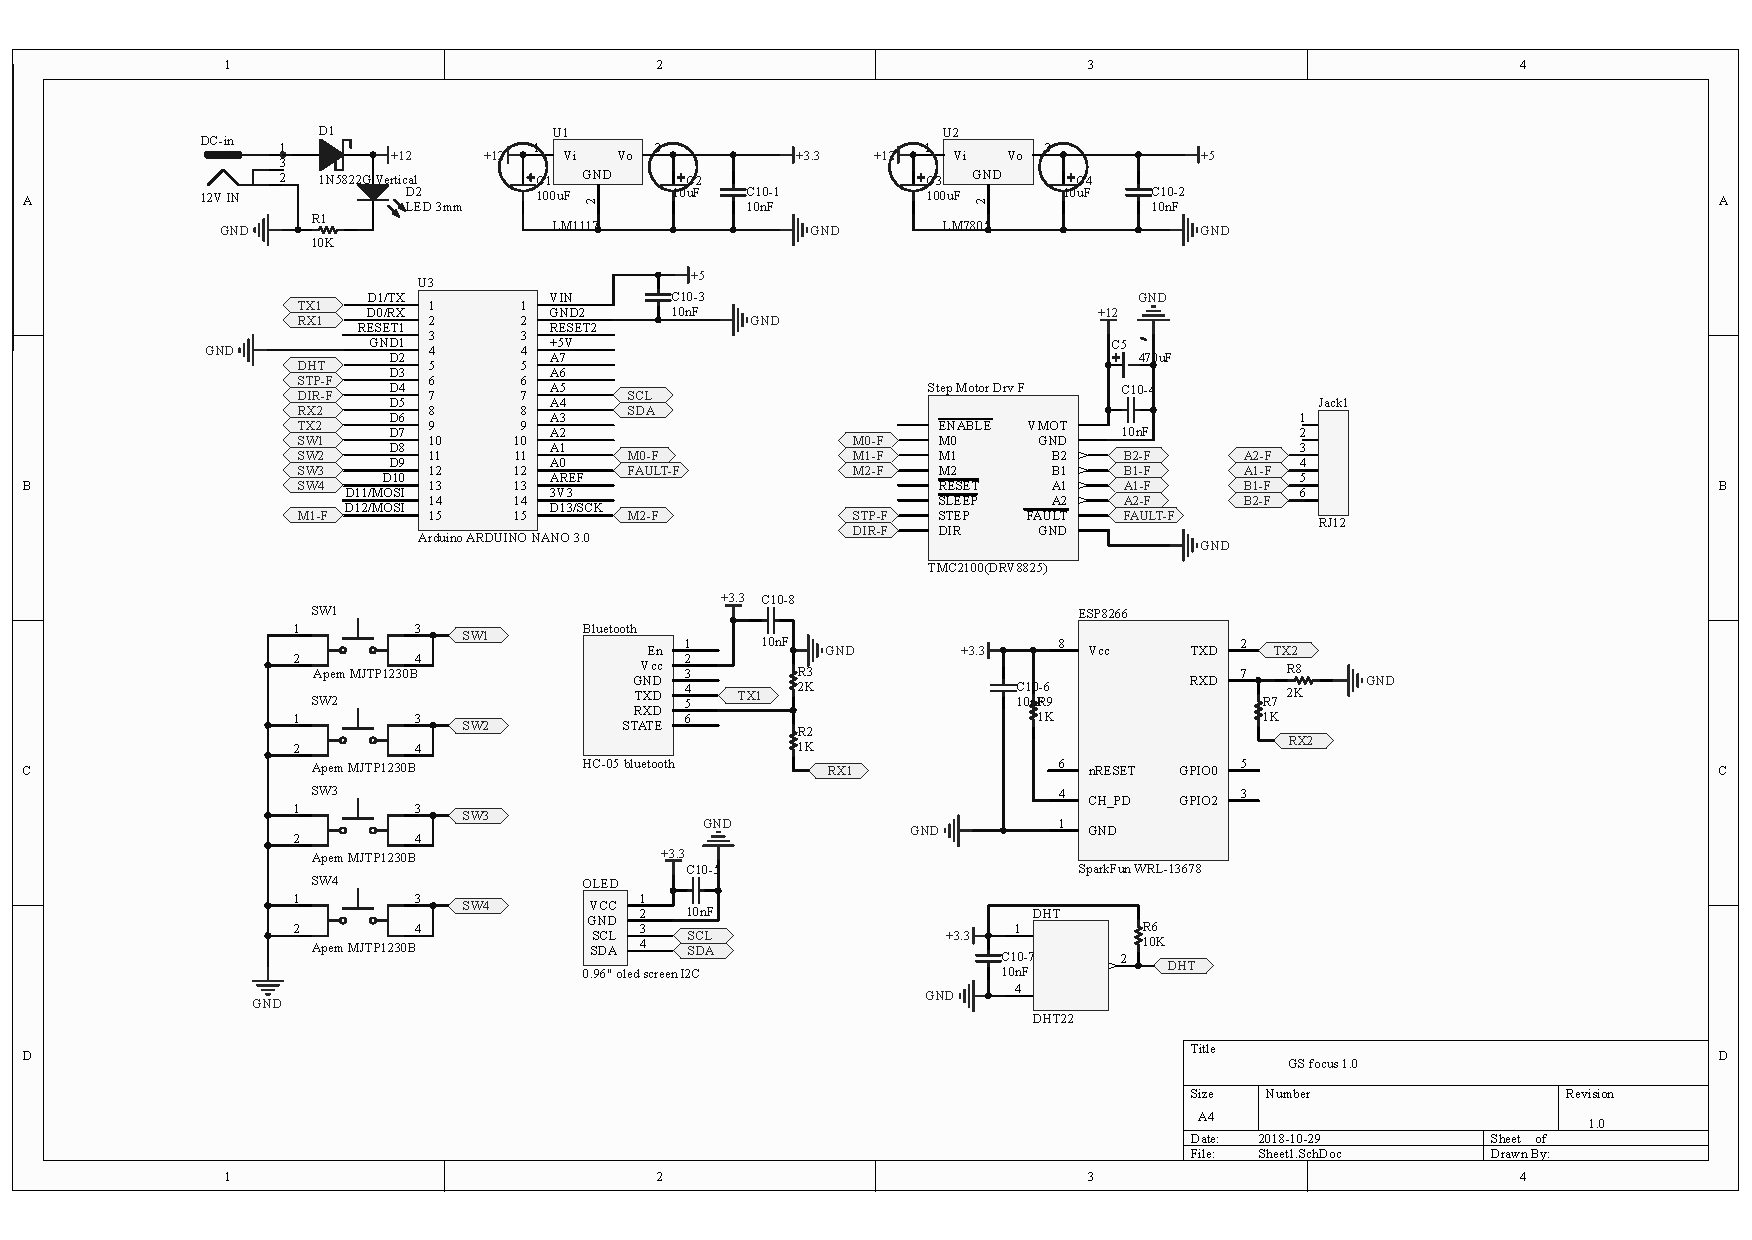
\includegraphics[width=1\linewidth]{Schematic_Prints}
	\caption{Circuitmaker를 이용하여 만든 차트}
	\label{fig:Schematic_Prints}
\end{wrapfigure}
생각보다 Circuitmaker 프로그램의 사용법을 숙지하는 데 오랜 시간이 걸렸기 때문에, 그사이에 진행된 연구에서는 만능기판에 여러 가지 부품들을 전선으로 연결하여 사용하는 방법을 택하였고, 연구가 진행되어 만능기판이 복잡해짐에 따라서 여러 프로그램의 도움을 받게 되었다.\\
연구 초기과정에서는 Arduino와 직접 연동이 가능한 ‘Fritzing’이라는 프로그램을 사용하였지만, 연구가 진행될수록 다른 부품들과 실제로 구현이 가능한 PCB 회로기판을 만들 수 있어야 했기 때문에 보편화한 PCB 회로제작 프로그램이면서 ‘협업’ 기능을 이용하여 동시에 수정이 가능한 ‘Circuitmaker’라는 프로그램을 사용하게 되었다.

\subsubsection{회로도 제작 시 주의 사항}

각 부품을 사용할 때에는 각 부품의 허용 전류와 같은 여러 가지 특징들을 생각하여 회로를 배선해야 한다. 예를 들어 WIFI 모듈인 ESP8266과 같은 경우 그 입력전압이 Arduino의 출력 전압인 5V가 아닌 3.3V이기 때문에 주의하여야 한다. 또한, 각 부품의 칩별로 제조한 회사의 data sheet를 참조하여 부품을 사용하면서 여러 가지 문제점들을 미리 방지하였다.\\
특히 5V를 3.3V로 바꾸는 과정에서는 전압 나눔 회로를 이용하여 전압을 나눌 수 있으나, 12V를 5V로 바꾸는 과정에서는 전류를 제어하는 것이 필요하므로 부득이하게 regulator를 사용하게 되었다.
\begin{figure}[ht]
	\begin{subfigure}{0.5\textwidth}
		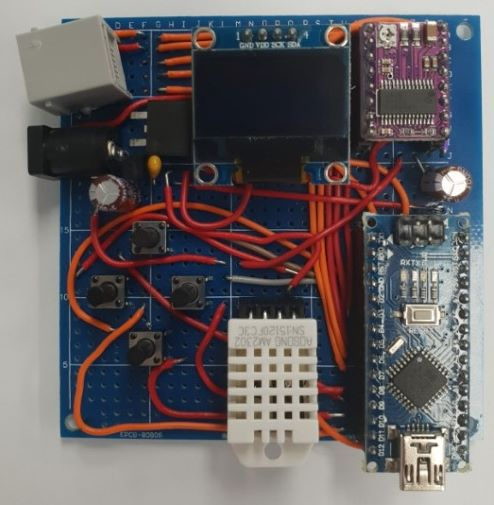
\includegraphics[width=0.9\linewidth, height=5cm]{circuit1} 
		\caption{만능기판으로 제작한 회로}
		\label{fig:circuit1}
	\end{subfigure}
	\begin{subfigure}{0.5\textwidth}
		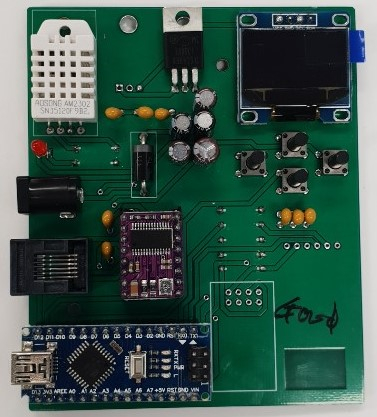
\includegraphics[width=0.9\linewidth, height=5cm]{pcbcircuit}
		\caption{PCB 기판으로 제작한 회로}
		\label{fig:pcbcircuit}
	\end{subfigure}
	\caption{제작한 회로도}
	\label{fig:image2}
\end{figure}

\subsubsection{펌웨어 개발}

Arduino를 이용하여 모터 초점 조절 장치를 만드는 데 필요한 기술들은 크게 4가지이다. 먼저, Arduino와 모터 드라이버(DRV8825)를 이용하여 모터를 돌릴 수 있어야 한다. 두 번째로, 스위치를 활용하여 모터의 움직임을 조절할 수 있게 하였다. 세 번째로, 모터를 조절한 것을 노트북에 연결되지 않고 12V의 외부전원만 연결된 상황에서도 모터가 얼마나 돌아갔는지를 확인할 수 있도록 모터가 얼마나 돌아가 있는지, 혹은 이로 인해 늘어난 경통의 길이가 얼마나 되는지 확인할 수 있도록 Arduino를 이용하여 OLED 판을 실행시켜 진행 상황을 확인할 수 있게 하여야 한다. 마지막으로, 모터가 너무 많이 돌아간 경우나 새로운 모터에 모터 컨트롤러를 사용하는 경우 이를 복원시키기 위해 표시된 숫자를 초기화하는 과정이 필요하다.\\
펌웨어를 개발하는 과정에서 위의 4가지 기능들이 들어갈 수 있도록 하였으며, 추가로 모터의 step을 옮기는 과정에서 다른 모터 포커서 컨트롤러들의 장점을 융합하여 편리하게 사용할 수 있도록 하였다.\\
먼저, 메뉴 기능을 통해 자신이 원하는 기능을 직접 선택할 수 있도록 하였다. 이를 통하여 모터를 연속적으로 돌리는 기능과 미리 설정한 일정 값 정보를 돌릴 수 있도록 지원한다. 특히 연속적으로 돌리는 기능은 버튼을 오래 누를수록 더 빠르게 돌 수 있도록 하여 효율성을 높였다. 또한, 모터를 돌리는 것뿐만이 아니라 자신이 얼마나 돌렸는지 표시하는 기능을 포함하였다.
\begin{figure}[h]
	\begin{subfigure}{0.5\textwidth}
		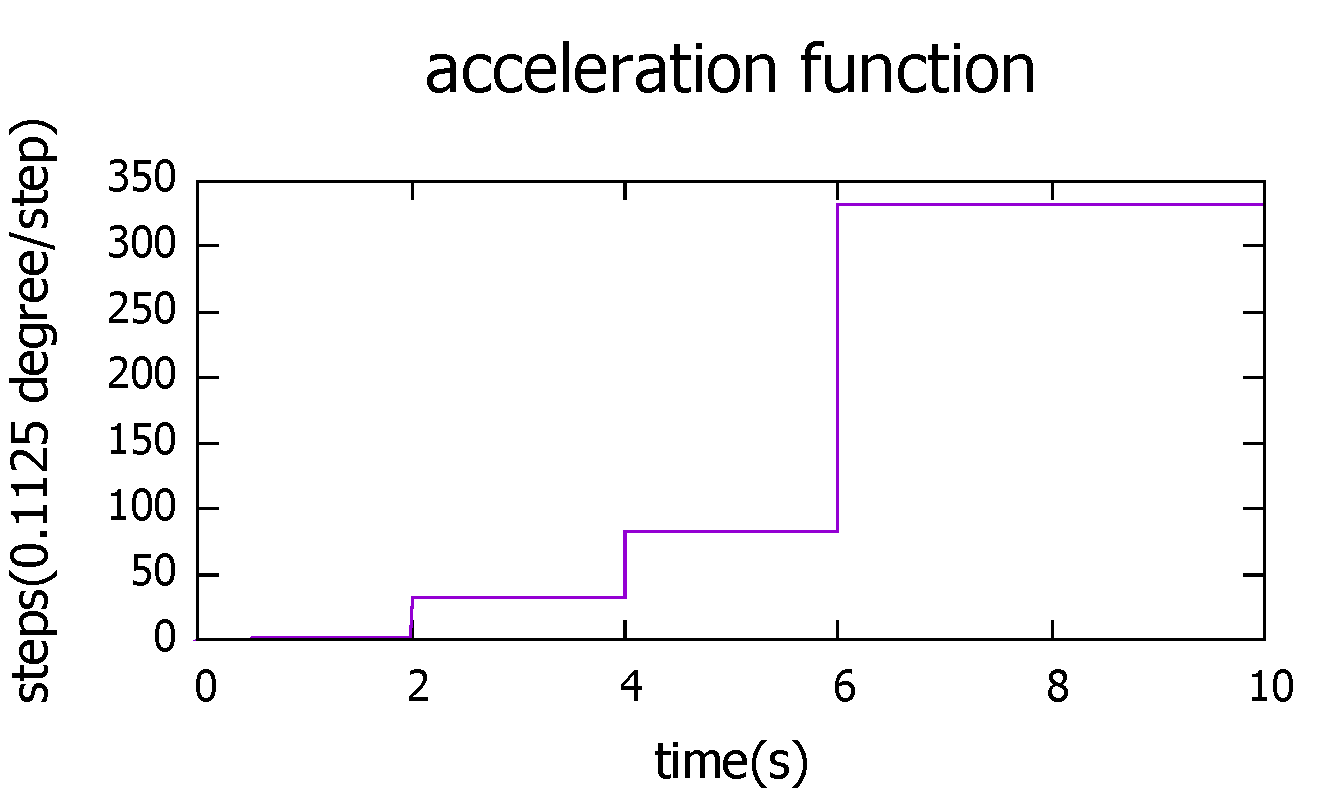
\includegraphics[width=0.9\linewidth, height=5cm]{function} 
		\caption{가속 기능}
		\label{fig:function}
	\end{subfigure}
	\begin{subfigure}{0.5\textwidth}
		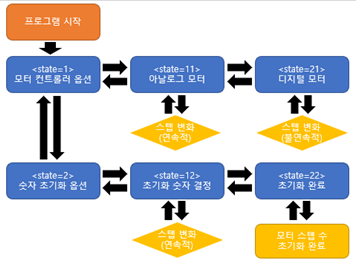
\includegraphics[width=0.9\linewidth, height=5cm]{algorithm}
		\caption{알고리즘}
		\label{fig:algorithm}
	\end{subfigure}
	\caption{펌웨어 설명}
	\label{fig:image3}
\end{figure}

\subsection{무선통신}

\subsubsection{블루투스}

\begin{wrapfigure}{l}{0.15\textwidth}
	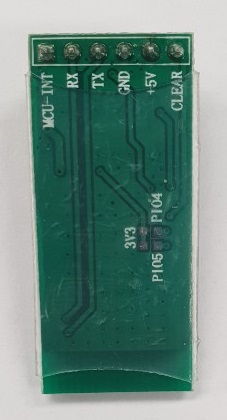
\includegraphics[width=1\linewidth]{HC06}
	\caption{HC06}
	\label{fig:HC06}
\end{wrapfigure}
블루투스는 보통 Arduino와 master-slave 관계를 맺어 정보를 서로 전달한다. OLED와 비슷하게 I2C 방식의 통신을 지원하는데, RX, TX 핀을 이용한 통신을 여러 가지를 실행하기 위해서는 “SoftwareSerial.h” 라이브러리를 이용하여 RX, TX 통신 핀을 여러 개로 따로 지정해주어야 한다.\\
본 연구에서 사용하는 모듈인 HC06 모델은 제품 스스로가 master가 될 수도 있고, slave로 설정될 수도 있다. (이와 비슷한 모델은 HC05는 slave 설정만 지원하기 때문에 아래에 서술할 방법을 사용하지 못함) 이를 발전시키면, 여러 개의 HC06을 활용하여서 한 모터 초점 조절 장치 컨트롤러에서 다른 모터 초점 조절 장치 컨트롤러로 정보를 서로 주고받을 수 있다.\\
블루투스는 페어링을 시키면 언제든지 사용할 수 있다는 장점이 있다.

\subsubsection{WIFI}

\begin{wrapfigure}{l}{0.06\textwidth}
	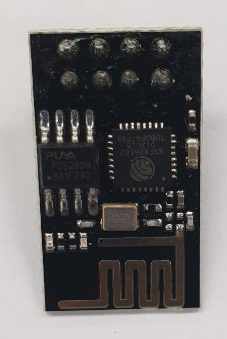
\includegraphics[width=1\linewidth]{ESP8266}
	\caption{ESP8266}
	\label{fig:ESP8266}
\end{wrapfigure}
가장 잘 알려져 있으며, 본 연구에서 사용하는 WIFI module인 ESP8266는 아두이노와 WIFI 연결을 가능하게 하여 준다. WIFI의 연결은 블루투스와 다르게 WIFI에 연결되어 있으면 언제든지 조절할 수 있다는 것이 큰 장점이며, IoT의 초기 모델로도 사용할 수 있다.\\
대부분의 WIFI module을 사용하려면 컴퓨터의 펌웨어를 업데이트해야 하므로 일반적으로 블루투스보다 사용이 어렵다. 

\subsection{ASCOM Protocol}

모터 초점 조절 장치를 활용하기 위해서는 별의 크기를 분석해서 돌려야 하므로 컴퓨터와의 연동을 위하여 초점 조절 장치의 ASCOM 드라이버를 C\# 코딩을 이용하여 제작한다. ASCOM 드라이버를 이용하면 카메라로부터 정보를 컴퓨터가 받아서 데이터를 분석하고, 이 분석한 데이터를 이용하여 모터를 어떻게 조절해야 할지 명령을 내리면 ASCOM 드라이버를 통해 정보를 전달하여 모터를 제어한 대로 조절이 가능하다.\\
현재 우리가 사용하는 프로그램은 ASCOM에서 만든 프로그램이고, ASCOM의 프로그램 대부분은 그 회사만의 표준 Protocol을 사용한다. 따라서 우리가 만드는 모터 초점 조절 장치 컨트롤러를 ASCOM Protocol에 따라 정보를 전달할 수 있도록 하면 일반 컴퓨터에 있는 ASCOM 프로그램을 이용하여 우리가 제작한 모터 초점 조절 장치 컨트롤러를 사용할 수 있도록 하는 것이 핵심이라고 할 수 있다.